\documentclass[acmsmall]{acmart}

\setcopyright{rightsretained}
\copyrightyear{2021}
\acmYear{2021}
\acmConference[HATRA '21]{Human Aspects of Types and Reasoning Assistants}{October 2021}{Chicago, IL}
\acmBooktitle{HATRA '21: Human Aspects of Types and Reasoning Assistants}

\newcommand{\squnder}[1]{\color{red}\underline{{\color{black}#1}}\color{black}}
\newcommand{\infer}[2]{\frac{\textstyle#1}{\textstyle#2}}
\newcommand{\erase}{\mathrm{erase}}
\newcommand{\evCtx}{\mathcal{E}}
\newcommand{\NIL}{\mathsf{nil}}
\newcommand{\TRUE}{\mathsf{true}}
\newcommand{\FALSE}{\mathsf{false}}
\newcommand{\NUMBER}{\mathsf{number}}
\newcommand{\ERROR}{\mathsf{error}}
\newcommand{\IF}{\mathsf{if}\,}
\newcommand{\THEN}{\,\mathsf{then}\,}
\newcommand{\ELSE}{\,\mathsf{else}\,}
\newcommand{\END}{\,\mathsf{end}}
\newcommand{\FUNCTION}{\mathsf{function}\,}
\newcommand{\RETURN}{\mathsf{return}\,}

\begin{document}

\title{Position Paper: Some Goals of the Luau Type System}

\author{Lily Brown}
\author{Andy Friesen}
\author{Alan Jeffrey}
\affiliation{
  \institution{Roblox}
  \city{San Mateo}
  \state{CA}
  \country{USA}
}

\begin{abstract}
  Luau is the scripting language that powers user-generated experiences on the
  Roblox platform. It is a statically-typed language with type inference based
  on the dynamically-typed Lua language. These types are used for providing
  editor assistance in Roblox Studio, the IDE for authoring Roblox experiences.
  Due to Roblox's uniquely heterogeneous developer community, Luau must operate
  in a somewhat different fashion than a traditional statically-typed language.
  In this paper, we describe some of the goals of the Luau type system,
  focusing on where the goals differ from those of other type systems.
\end{abstract}

\maketitle

\section{Introduction}

The Roblox~\cite{Roblox} platform allows anyone to create shared,
immersive, 3D experiences.  As of July 2021, there are
approximately 20~million experiences available on Roblox, created
by 8~million developers.  Roblox creators are often young. For
example, there are over 200~Roblox kids' coding camps in 65~countries
listed by the company as education resources~\cite{AllEducators}.
The Luau programming language~\cite{Luau} is the scripting language
used by creators of Roblox experiences. Luau is derived from the Lua
programming language~\cite{Lua}, with additional capabilities,
including a type inference engine.

This paper will discuss some of the goals of the Luau type system, such
as supporting goal-driven learning, non-strict typing semantics, and
mixed strict and non-strict types.  Particular focus is placed on how
these goals differ from traditional type systems' goals.

\section{Human Aspects}
\subsection{Heterogeneous developer community}

Quoting a Roblox 2020 report \cite{RobloxDevelopers}:
\begin{itemize}
\item Adopt Me! now has over 10 billion plays and surpassed 1.6 million concurrent users earlier this year.
\item Piggy, launched in January 2020, has close to 5 billion visits in just over six months.
\item There are now 345,000 developers on the platform who are monetizing their games.
\end{itemize}
This demonstrates the heterogeneity of the Roblox developer community:
developers of experiences with billions of plays are on the same
platform as children first learning to code. Moreover, \emph{both of
these groups are important}. The professional development studios
bring high-quality experiences to the platform, and the beginning creators
contribute to the energetic creative community, forming the next generation of developers.

\subsection{Goal-driven learning}

Goal: \emph{support learning how to perform specific tasks organically}

All developers are goal-driven, but this is especially true for
learners. A learner will download Roblox Studio with an
experience in mind, such as designing an obstacle course (an ``obby'')
to play in with their friends.

The user experience of developing a Roblox experience is primarily a
3D interactive one, seen in Fig.~\ref{fig:studio}(a). The user designs
and deploys 3D assets such as terrain, parts and joints, providing
them with physics attributes such as mass and orientation. The user
can interact with the experience in Studio, and deploy it to a Roblox
server so anyone with the Roblox app can play it. Physics, rendering
and multiplayer are all immediately accessible to creators.

\begin{figure}
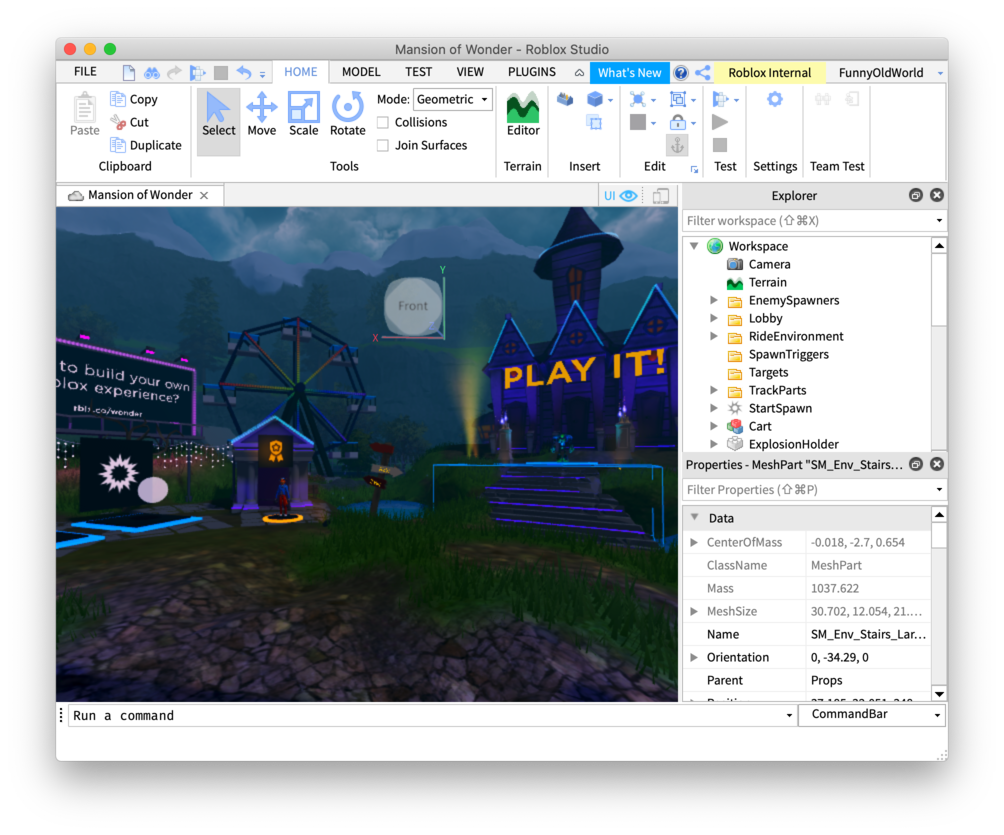
\includegraphics[width=0.48\textwidth]{studio-mow.png}
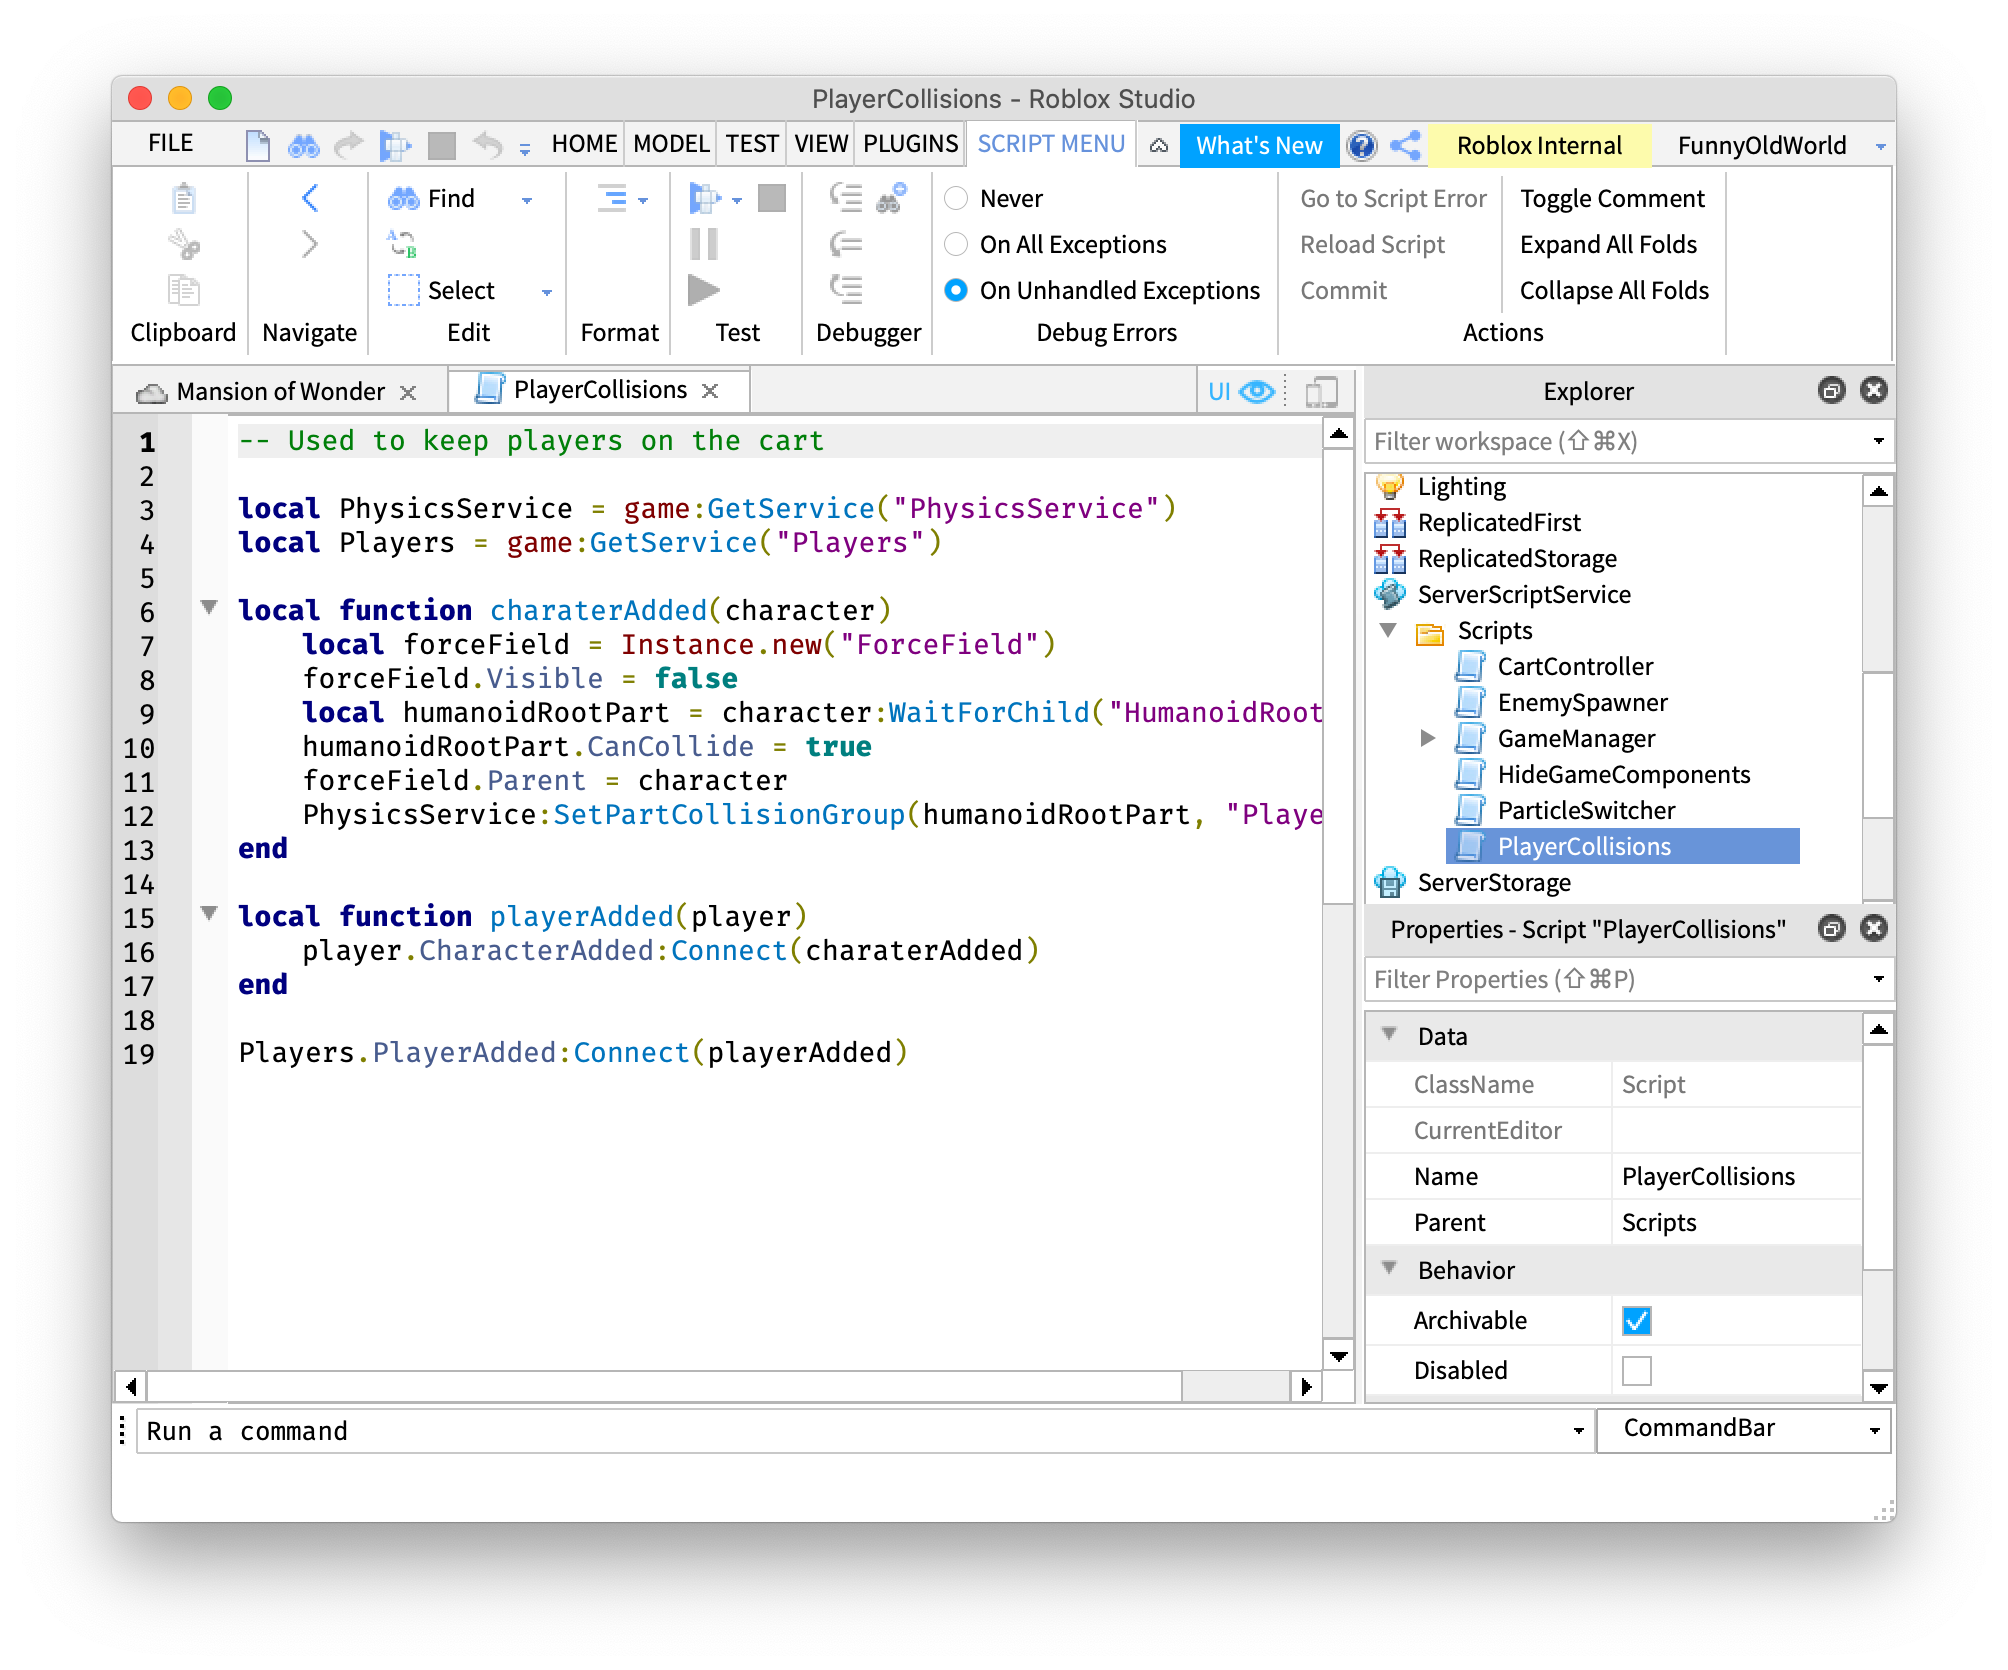
\includegraphics[width=0.48\textwidth]{studio-script-editor.png}
\caption{Roblox Studio's 3D environment editor (a), and script editor (b)}
\label{fig:studio}
\end{figure}

At some point during experience design, the experience creator has a need
which can't be met by the physics engine alone, such as ``The stairs should
light up when a player walks on them'' or ``a firework is set off
every few seconds.'' At this point they will discover the script
editor, seen in Fig.~\ref{fig:studio}(b).

This onboarding experience is different from many initial exposures to
programming, in that by the time the user first opens the script
editor, they have already built much of their creation, and have a
very specific concrete aim. As such, Luau must allow users to perform a
specific task with a minimum of ``boilerplate'' code.

\subsection{Type-driven development}

Goal: \emph{enable users to leverage types in their development process}

Professional development studios are also goal-directed (though the
goals may be more abstract, such as ``decrease user churn'' or
``improve frame rate'') but have additional needs:
\begin{itemize}

\item \emph{Code planning}:
  code spends much of its time in an incomplete state, with holes
  that will be filled in later.

\item \emph{Code refactoring}:
  code evolves over time, and it is easy for changes to
  break previously-held invariants.

\item \emph{Defect detection}:
  code has errors, and detecting these at runtime (for example by crash telemetry)
  can be expensive and recovery can be time-consuming.
  
\end{itemize}
Detecting defects ahead-of-time is a traditional goal of type systems,
resulting in an array of techniques for establishing safety results,
surveyed for example in~\cite{TAPL}. Supporting code planning and
refactoring are some of the goals of \emph{type-driven
development}~\cite{TDDIdris} under the slogan ``type, define,
refine''.  For example, a common use of type-driven development is renaming a
property, which is achieved by changing the name in one place,
and then fixing the resulting type errors---once the type system stops
reporting errors, the refactoring is complete.

To help support the transition from novice to experienced developer,
types are introduced gradually, through API documentation and type discovery.
Type inference provides many of the benefits of type-driven development
even to creators who are not explicitly providing types.

\section{Types}
\subsection{Infallible types}

Programs spend much of their time under development in an ill-typed or incomplete state, even if the
final artifact is well-typed. Tools should support this by \emph{providing type information even for ill-typed programs}.
An analogy is infallible parsers, which perform error recovery and provide an AST for all input texts.

Program analysis can still flag type errors, which may be presented
to the user with red squiggly underlining. Formalizing this, rather
than a judgment
$\Gamma\vdash M:T$, for an input term $M$, there is a judgment
$\Gamma \vdash M \Rightarrow N : T$ where $N$ is an output term
where some subterms are \emph{flagged} as having type errors, written $\squnder{N}$. Write $\erase(N)$
for the result of erasing flaggings: $\erase(\squnder{N}) = \erase(N)$.

%% For example the usual
%% type rules for field access becomes:
%% \[
%%   \infer{
%%     \Gamma \vdash M \Rightarrow M' : T
%%   }{
%%     \Gamma \vdash M.\ell \Rightarrow M'.\ell : U
%%   }
%%   [
%%     T = \{ \overline{\ell:U} \} \mbox{ and } (\ell:U) \in (\overline{\ell:U})
%%   ]
%% \]
%% but there is also a rule for unsuccessful field access:  
%% \[
%%   \infer{
%%     \Gamma \vdash M \Rightarrow M' : T
%%   }{
%%     \Gamma \vdash M.\ell \Rightarrow \squnder{M'.\ell} : U
%%   }
%%   [
%%     T = \{ \overline{\ell:U} \} \mbox{ implies } \ell \not\in \overline{\ell}
%%   ]
%% \]
%% In this type rule, $U$ is unconstrained.

The goal of infallible types is that every term can be typed:
\begin{itemize}
\item \emph{Typability}: for every $M$ and $\Gamma$,
  there are $N$ and $T$ such that $\Gamma \vdash M \Rightarrow N : T$.
\item \emph{Erasure}: if $\Gamma \vdash M \Rightarrow N : T$
  then $\erase(M) = \erase(N)$ 
\end{itemize}
Some issues raised by infallible types:
\begin{itemize}
\item Which heuristics should be used to provide types for flagged programs? For example, could one
  use minimal edit distance to correct for spelling mistakes in field names?
\item How can we avoid cascading type errors, where a developer is
  faced with type errors that are artifacts of the heuristics, rather
  than genuine errors?
\item How can the goals of an infallible type system be formalized?
\end{itemize}
\emph{Related work}:
there is a large body of work on type error reporting
(see, for example, the survey in~\cite[Ch.~3]{TopQuality})
and on type-directed program repair
(see, for example, the survey in~\cite[Ch.~3]{RepairingTypeErrors}),
but not type repair, or on
the semantics of programs with type errors. Many compilers perform
error recovery during typechecking, but do not provide a semantics
for programs with type errors.

\subsection{Strict types}

Goal: \emph{no false negatives.}

For developers who are interested in defect detection, Luau provides a \emph{strict mode},
which acts much like a traditional, sound, type system. This has the goal of ``no false negatives''
where any possible run-time error is flagged. This is formalized using:
\begin{itemize}
\item \emph{Operational semantics}: a reduction judgment $M \rightarrow N$ on terms.
\item \emph{Values}: a subset of terms representing a successfully completed evaluation.
\end{itemize}
Error states at runtime are represented as stuck states (terms that are not
values but cannot reduce), and showing that no well-typed program is
stuck. This is not true if typing is infallible, but can fairly
straightforwardly be adapted. We extend the operational semantics to flagged terms,
where $M \rightarrow M'$ implies $\squnder{M} \rightarrow \squnder{M'}$, and
for any value $V$ we have $\squnder{V} \rightarrow V$, then show:
\begin{itemize}
\item \emph{Progress}: if ${} \vdash M \Rightarrow N : T$, then $N \rightarrow N'$ or $N$ is a value or $N$ has a flagged subterm.
\item \emph{Preservation}: if ${} \vdash M \Rightarrow N : T$ and $N \rightarrow N'$ then  $M \rightarrow^*M'$ and ${} \vdash M' \Rightarrow N' : T$.
\end{itemize}
Some issues raised by infallible types:
\begin{itemize}
\item How should the judgments and their metatheory be set up?
\item How should type inference and generic functions be handled?
\item Is the operational semantics of flagged values
  ($\squnder{V} \rightarrow V$) the right one?
\item Will higher-order code require wrappers on functions? 
\end{itemize}
\emph{Related work}: gradual typing and blame analysis, e.g.~\cite{GradualTyping,WellTyped,Contracts}

\subsection{Nonstrict types}

Goal: \emph{no false positives.}

For developers who are not interested in defect detection, type-driven
tools and techniques such as autocomplete, API documentation
and support for refactoring can still be useful.
For such developers, Luau provides a
\emph{nonstrict mode}, which we hope will eventually be useful for all
developers.  The non-strict typing mode is particularly useful when
adopting Luau types in pre-existing code, which was not authored with
the type system in mind.  Non-strict mode does \emph{not} aim for
soundness, but instead has the goal of ``no false positives``, in the
sense that any flagged code is guaranteed to produce a runtime error
when executed.

On the face of it, this is undecidable, since a program such as
$(\IF f() \THEN \ERROR \END)$ will produce a runtime error when $f()$ is
$\TRUE$, but we can aim for a weaker property, that all flagged code
is either dead code or will produce an error. Either of these is a
defect, so deserves flagging, even if the tool does not know
which reason applies.

We can formalize this by defining an \emph{evaluation context}
$\evCtx[\bullet]$, and saying $M$ is \emph{incorrectly flagged}
if it is of the form $\evCtx[\squnder{V}]$. We can then define:
\begin{itemize}
\item \emph{Correct flagging}: if ${} \vdash M \Rightarrow N : T$
  then $N$ is correctly flagged.
\end{itemize}
Some issues raised by nonstrict types:
\begin{itemize}

\item Under this definition, any function that will terminate is unflagged, so
  flagging will often move from function definitions to call sites.

\item This definition will not allow an unchecked use of an optional value
  to be flagged, for example if $f() : \NUMBER?$ (meaning $f$ may optionally return a number)
  then a strict type system can flag $1 + f()$ but a nonstrict one cannot.

\item Property update of tables in languages like Luau always succeeds
  (the property is inserted if it did not exist), and so functions which
  update properties cannot be flagged.

\item Does nonstrict typing require whole program analysis,
  to find all the possible types a property might be updated with?

\item The natural formulation of function types in a nonstrict setting
  is that of~\cite{???}: if $f: T \rightarrow U$ and $f(V) \rightarrow^* W$
  then $V:T$ and $W:U$. This formulation is \emph{covariant} in $T$,
  not \emph{contavariant}; what impact does this have?
  
\end{itemize}
\emph{Related work}: success types~\cite{SuccessTyping} and incorrectness logic~\cite{IncorrectnessLogic}.

\subsection{Mixing types}

Goal: \emph{support mixed strict/nonstrict development}.

Like every active software community, Roblox developers share code
with one another constantly.  First- and third-party developers alike
frequently share entire software packages written in Luau.  To add to
this, many Roblox experiences are authored by a team.  It is therefore
crucial that we offer first-class support for mixing code written in
strict and nonstrict modes.

Some questions raised by mixed-mode types:
\begin{itemize}

\item How much feedback can we offer for a nonstrict script that is
  importing strict-mode code?

\item In strict mode, how do we talk about values and types that are
  drawn from nonstrict code?

\item How can we combine the goals of strict and nonstrict types?

\item Can we have strict and non-strict mode infer the same types,
  only with different flagging?

\item Is strict-mode code sound when it relies on non-strict code,
  which has weaker invariants?

\end{itemize}
\emph{Related work}: this appears to be an under-explored area.

\section{Conclusions}

In this paper, we have presented some of the goals of the Luau type
system, and how they map to the needs of the Roblox creator
community. We have sketched what a solution might look like; all that
remains is to draw the owl~\cite{HowToDrawAnOwl}.

\bibliographystyle{ACM-Reference-Format} \bibliography{bibliography}

\end{document}
